%
% Advanced Robotics submission
% Internal models of reaching and grasping
% Castellini, Orabona, Metta, Sandini
%

\documentclass{arsubmit}
\usepackage{graphicx}
\usepackage{amsmath}
\usepackage[psamsfonts]{amssymb}

\def\RR{\mathbb{R}}
\def\NN{\mathbb{N}}
\def\xx{\mathbf{x}}
\def\ww{\mathbf{w}}
\def\aa{\mathbf{\alpha}}
\def\bb{\mathbf{\beta}}
\def\ee{\mathbf{e}}
\def\dd{\mathbf{d}}
\def\mdd{\tilde{\dd}}
\def\b{\mathcal{B}}
\def\d{\mathcal{D}}

\title{Internal models of reaching and grasping}

\author{Claudio Castellini \and Francesco Orabona \and Giorgio Metta \and Giulio Sandini}

\date{\small \it{
LIRA-Lab and Italian Institute of Technology\\
Genoa, Italy\\
{\tt contact: pasa@liralab.it}
}}

\begin{document}

\maketitle

\begin{abstract}
Grasping is one of the most challenging tasks in advanced robotics...

\end{abstract}

{\it keywords}: human movement, sensing system for daily life,
sensorimotor pattern sand symbol correlation acquisition, motion
capturing systems and its application

\section{INTRODUCTION}
\label{sec:introduction}
It is reasonably well established that the brain stores internal models of action
either because they are required to control movement or, as it has been determined
more recently, to interpret the movement of others \cite{kawato-99, wolpert-03, 
mussaivaldi-00, lackner-98}. 
There is a large body of literature that links observation of action to action 
execution as for example the study of the motor system conducted by Rizzolatti and 
colleagues in relatively recent years \cite{rizzolatti-04,gallese-96,rizzolatti-01}. 

In the monkey, premotor area F5 has been particularly well studied and it is in fact the 
location where ``mirror neurons'' were first identified. In this respect, mirror neurons 
are the quintessential correlate of internal models since they are activated 
both when executing a specific grasping action and when observing a congruent action 
being executed by another individual (or the experimenter) \cite{fadiga-00}.

In a study by Umilt\'a et al. \cite{umilta-01} the response of mirror neurons to the observation of
actions that terminate behind a screen has been investigated. In this case, the authors analyzed 
mirror neurons in situations where the final part of the action was occluded by an opaque 
screen with the monkey knowing of the presence/absence of an object to be grasped. As long
as the object was shown to the monkey, the brain could easily supply the missing
visual information by rehearsing the internal model of the action. The control experiment, 
in this case, was that of an identical hand kinematics, an identical screen but the absence of 
the target object, that is, identical visual stimulation apart from the knowledge of the 
presence of the object. Elsewhere it has been also shown that the presence of an object is 
required to elicit the mirror neurons response in the monkey \cite{gallese-96}.

{\em A posteriori}, given these results, it is easy to see how the presence of a target 
object and its geometrical properties strongly constrain the type of grasp and the approach 
to the object, and that, as a consequence, the brain might need to include this information when 
planning an appropriate course of action. 
As we mentioned earlier, in the monkey these constraints are so strong that mirror neurons do not 
fire unless the goal of the action is clearly perceivable. The brain codes for the object-motor 
identity in part via another class of F5 visuomotor neurons called ``canonical neurons'' (for a 
discussion see for example \cite{metta-06}). 
To complete the ``picture'', the work of Graziano, Hu, and Gross \cite{graziano-97} has shown that 
the presence of object is coded in the ventral premotor cortex and maintained even when the 
object is no longer visible as long as there is evidence for its presence at a particular
location.

Relevant to this discussion, the work of Fogassi et al. \cite{fogassi-05} contributed to the 
identification of mirror neurons in the parietal cortex (inferior parietal lobule), which are 
thought to be related to the decoding of the intentions of others. Contextual information 
which links the enacted action to its final goal seems to be implicated in this type of neural 
response. The presence of objects is a clear contextual cue.

In humans, it has been demonstrated that the activation of brain areas correlated to 
action observation is not simply a perceptual effect but rather the activation of
a precise sensorimotor model which includes for example the hand kinematics \cite{pozzo-06}.
 
Accordingly, Fadiga et al. \cite{fadiga-99,vargas-04} have shown that motor imagery changes
the excitability of the cortico-spinal connections specifically to the imagined action, that is, 
imagining a motor task causes the under-threshold activation of the same neural pathways 
required to execute the task. This under-threshold activation was revealed 
by transcranial magnetic stimulation. In a conceptually similar experiment 
\cite{fadiga-05}, the excitability of cortico-spinal pathways was also examined as a consequence 
of the actual sensory input. In summary, the motor system is similarly activated 
when acting in first person, when imagining an action, or when watching somebody else's action.

% note: it'd be nice to examine the difference with presence/absence of the object in
% humans using the TMS.

Jeannerod \cite{jeannerod-88}, for example, goes in great length in showing how plausible is the fact that
mental imagery uses the same internal models used by actual action generation. It is known in 
this respect that the time required to simulate an action is the same that is required to 
execute that action \cite{sirigu-96}. For a review refer to \cite{jeannerod-99}.




[SAY SOMETHING ABOUT IMITATION, TELEOPERATION and PROSTHETIC]

VISION -> MOTOR, shown by ourselves.

\section{SUPPORT VECTOR MACHINES}
\label{sec:svm}
Assume $\{\xx_i,y_i\}_{i=1}^l$, with $\xx_i \in \RR^m$ and $y_i \in
\{-1,1\}$, is a set of samples drawn from an unknown probability
distribution. The problem is to approximate it in order to classify
more data coming from the same source to the best extent
possible. Assuming the data are linearly separable, according to the
standard approach, a \emph{separating hyperplane} in $\RR^m$ is sought
for:

\begin{equation} \label{eqn:dec}
  f(\xx) = sgn(\ww\cdot\xx + b)
\end{equation}

\noindent with $\ww \in \RR^m$ and $b \in \RR$. In this case, the
hyperplane must respect the constraints $y_i(\ww\cdot\xx_i + b)-1\geq
0$, for all $i = 1,\ldots,l$ (from now on, this will be implicit
whenever a subscript $i$ appears free in a formula). In the general,
more likely and realistic case in which the data are not linearly
separable, we introduce $l$ slack variables $\xi_i$ and rather require
that $y_i(\ww\cdot\xx_i + b)-1+\xi_i\geq 0$, with $\xi_i \geq 0$. In
order to find such a hyperplane, we wish to maximise the hyperplane's
distance from both groups of samples (\emph{margin}). The margin is
easily determined to be $\frac{2}{||\ww||}$, so we are left with the
problem of minimising $||\ww||$ subject to the above constraints. The
problem is then usually solved minimising the following expression:

\begin{equation} \label{eqn:svm_primal}
  \min_{\ww} \left( ||\ww||^2 + C \sum_{i=1}^l \xi_i \right)
\end{equation}

\noindent subject to the constraints

\begin{eqnarray} \label{eqn:svm_constr}
  y_i (\ww\cdot\xx_i + b) & \geq & 1-\xi_i \\
                    \xi_i & \geq & 0 \nonumber
\end{eqnarray}

\noindent where $C \in \RR$ is a positive weight coefficient. Since
both the problem and the constraints are convex,
(\ref{eqn:svm_primal}) and (\ref{eqn:svm_constr}) can be compactly
expressed in Lagrangian form by introducing $l$ pairs of coefficients
$\alpha_i, \mu_i$ and then minimising the objective function

\begin{equation} \label{eqn:lp1}
  L_P =
      \frac{1}{2} ||\ww||^2
    - \sum_{i=1}^l \alpha_i \left(y_i (\ww\cdot\xx_i+b) - 1 + \xi_i \right)
    + C \sum_{i=1}^l \xi_i
    - \sum_{i=1}^l \mu_i \xi_i
\end{equation}

\noindent subject to the constraints that $\alpha_i,\mu_i\geq 0$. By
using the extremum conditions for $\ww$ and $b$, that is,
$\nabla_{\ww,b} L_P = 0$, one finds that

\begin{equation} \label{eqn:w1}
  \ww = \sum_{i=1}^l \alpha_i y_i \xx_i
\end{equation}

\noindent which, substituted in Equation (\ref{eqn:dec}), gives

\begin{equation} \label{eqn:lin_sol}
  f(\xx) = sgn \left( \sum_{i=1}^l \alpha_i y_i \xx \cdot \xx_i + b \right)
\end{equation}

Notice that, in the last Equation, the $\xx$'s only appear in the form
of inner products; in order to boost the expressive power of SVMs
then, the $\xx_i$s are usually mapped to a highly, possibly
infinite-dimensional space (the \emph{feature space}) via a
non-linear mapping $\Phi(\xx)$; the core of the SVM becomes then the
so-called \emph{kernel function} $K$ such that $K(\xx_1,\xx_2) =
\Phi(\xx_1)\cdot\Phi(\xx_2)$. This idea is called \emph{kernel trick}
and is standard in literature; it avoids the necessity of explicitly
knowing $\Phi$. Equation (\ref{eqn:lin_sol}) then becomes

\begin{equation} \label{eqn:sol}
  f(\xx) = sgn \left( \sum_{i=1}^l \alpha_i y_i K(\xx,\xx_i) + b \right)
\end{equation}

After training, that is after the minimisation of $L_P$, some of the
$\alpha_i$s (actually most of them in many practical applications) are
zero; those $\xx_i$s for which this does \emph{not} hold are somehow
crucial to the solution and are called \emph{support vectors}, hence
the name of the approach. This phenomenon is known as
\emph{sparseness} of the solution, meaning that only a subset of the
training data is usually really needed to build it.


\section{MATERIALS AND METHODS}
\label{sec:exp_desc}
In this Section we detail the process of gathering data from human
subjects and processing them in order to make them suitable for
analysis by a machine learning system. In particular, we address the
problem of building a \emph{training set}, that is, a set of data
effectively representing, for each user and object considered, the
grasping process, that could be used to train the system.

\subsection{Experimental Setup}

\subsubsection*{Devices}

We collected data using a $22$-sensors Immersion CyberGlove for the
hand posture \cite{cyberglove}, an Ascension Flock-Of-Birds (FoB) for
the hand position \cite{fob} and a Force Resistor Sensor (FSR) to
detect the contact moment with the object. Figure \ref{fig:devices}
shows the devices, as worn by a subject.

\begin{figure}[htbp]
  \begin{center}
    \begin{tabular}{cc}
      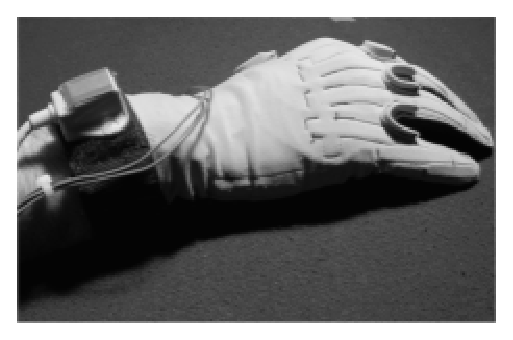
\includegraphics[width=0.45\linewidth]{devices1.eps} &
      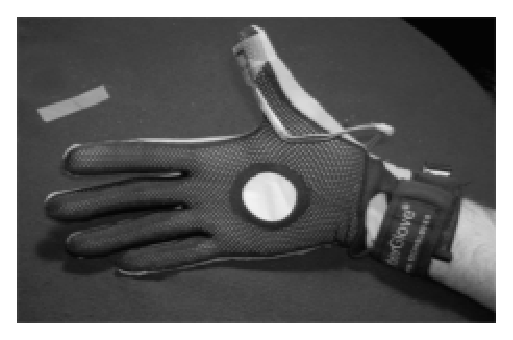
\includegraphics[width=0.45\linewidth]{devices2.eps} \\
      $(a)$ & $(b)$
    \end{tabular}
    \caption{The devices used for the experiment, as worn by a
    subject: $(a)$ the CyberGlove, with the Flock-of-Birds just above
    the subject's wrist; $(b)$ the Force Resistor Sensor attached to
    the subject's thumb.}
    \label{fig:devices}
  \end{center}
\end{figure}

The CyberGlove was worn by the subject on the right hand. The device
returns $22$ $8$-bit numbers linearly related to the angles between
the ends of the sensors and roughly indicating the angles between the
subject's hand joints; the sensors are embedded in the glove in order
for them to be adherent to the subject's skin. The resolution of the
sensors is on average about $0.5$ degree \cite{cyberglove}, but the
noise associated with the sensors has been experimentally determined
to be $1.1$ on average and $3$ at the maximum \cite{212431}. The
sensors describe the position of the three phalanxes of each finger
(for the thumb, rotation and two phalanxes), the four finger-to-finger
abductions, the palm arch, the wrist pitch and the wrist yaw.

The FoB was firmly mounted on the CyberGlove, just above the subject's
wrist, with the $X/Y$ plane being parallel to the palm plane in the
resting position. The device returns $6$ double-precision numbers
describing the position ($x$, $y$ and $z$ in inches) and rotation
(azimuth, elevation and roll in angles) of the sensor with respect to
a magnetic basis mounted about one meter away from the subject. The
FoB's resolution is $0.1$ inches and $0.5$ degrees \cite{fob}.

Lastly, the FSR was mounted on the subject's thumb. It returns a
$32$-bit number approximately inversely proportional to the pressure
applied to the surface of the sensor. We only used the FSR as an
on-off indicator of when the subject made contact with the object.

All data were collected, synchronised, and saved in real time at a
frequency of $50$Hz.

\subsubsection*{Subjects}

Eleven subjects, four females and seven males aged $24$ to $34$ of
different nationalities, joined the experiment. They were all
right-handed and fully able-bodied, and were given initially some
knowledge of the aim of the experiment.

\subsubsection*{Method}

The subjects were asked to sit confortably in front of a clean
workspace of about one squared meter, at the center of which an object
was placed, in a predefined position. The subjects were then asked to
wear the devices and choose a resting position for their right hand
and arm. They were then instructed to grasp the object with their
right hand any way they wanted, not necessarily the same way each
time, keeping a ``natural'' attitude. After grasping the object, they
had to drop it somewhere else in the workspace, and then return their
right hand and arm in the initial resting position. Subsequently, they
had to use their left hand to reposition the object roughly in the
same place it was before.

We first had the subjects do a trial run of the experiment, in order
for them to gain confidence in the setup. A beeping sound was heard
each time the subject made contact with the object (that is, each time
the FSR signalled a significant change), and they were asked to try
and hear the beep each time they grasped the object. Although this
ruled out grasps which made no use of the thumb, it enabled us to
better gather the contact points.

After the trial run, subjects were asked to repeat the
grasp/drop/reposition procedure $120$ times per each object. We will
call both this procedure and the data time sequence gathered during
the procedure, a \emph{session}. We employed, in turn, three objects:
a beer can, a scotch tape roll and a mug (Figure \ref{fig:objects}
shows the objects). The objects were chosen so that each of them could be
grasped in several different ways, but with a certain degree of
overlapping, e.g., both the beer can and the mug could be grasped
cylindrically, but only the mug could be grasped using the handle.

\begin{figure}[htbp]
  \begin{center}
    \begin{tabular}{ccc}
      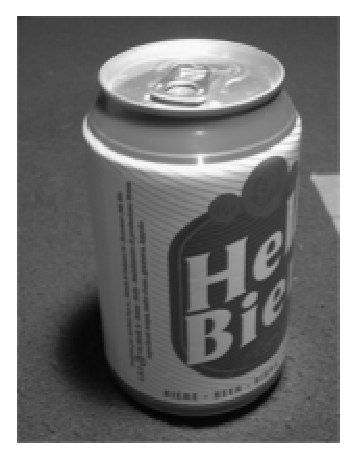
\includegraphics[height=0.2\textheight]{beer.eps} &
      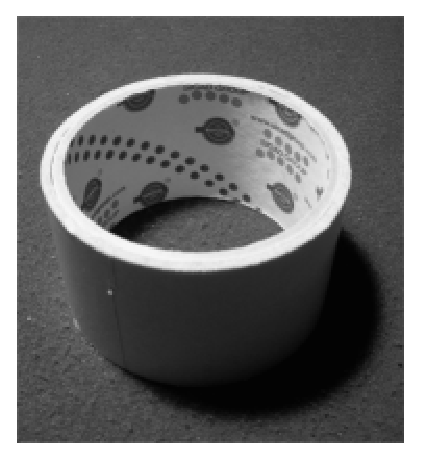
\includegraphics[height=0.2\textheight]{scotch.eps}  &
      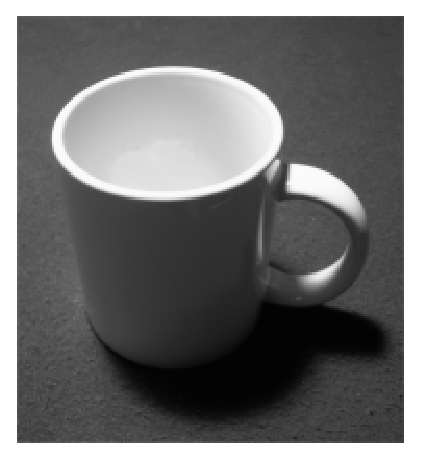
\includegraphics[height=0.2\textheight]{mug.eps} \\
      $(a)$ & $(b)$ & $(c)$
    \end{tabular}
    \caption{The objects used in the experiment: a beer can $(a)$, a
    scotch tape roll $(b)$ and a mug $(c)$.}
    \label{fig:objects}
  \end{center}
\end{figure}

Each experiment employed one subject and consisted of six sessions:
first the can, then the roll and then the mug, all of this two times,
for an approximate total of $720$ grasps per subject, $240$ per
object. The numbers are not precise since now and then the subjects
would grasp without properly activating the FSR. This problem has been
corrected in the batch analysis of data.

Each experiment lasted $35$ to $56$ minutes depending on the subject's
confidence and speed; although almost no subjects reported tiredness,
we allowed for rest between each session. It was reported by almost
every subject that the experiment became rapidly boring, which lets us
claim that almost all grasps were done in a natural, almost
unconscious way. Figure \ref{fig:setup} shows the main phases of the
experiment.

\begin{figure}[htbp]
  \begin{center}
    \begin{tabular}{ccc}
      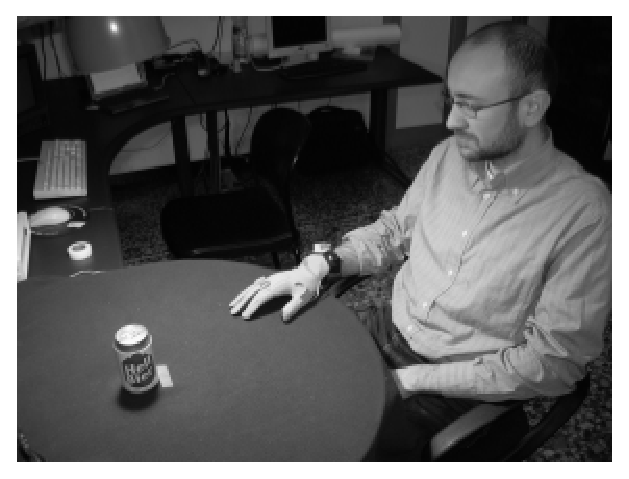
\includegraphics[width=0.3\linewidth]{exp1.eps} &
      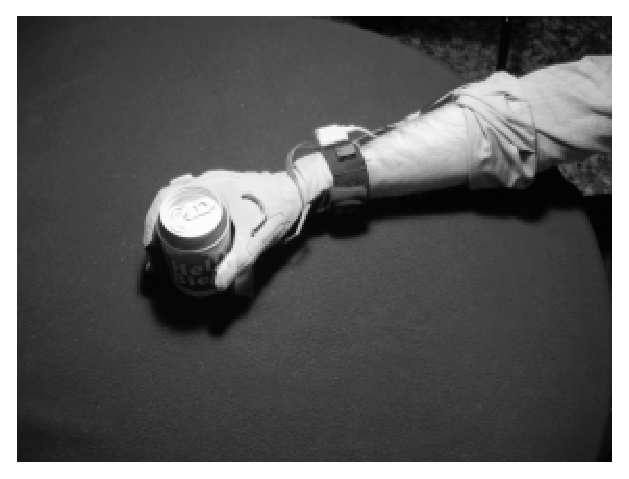
\includegraphics[width=0.3\linewidth]{exp2.eps}  &
      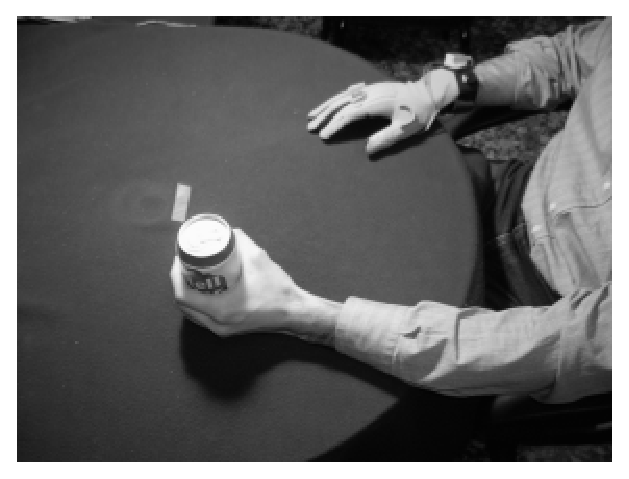
\includegraphics[width=0.3\linewidth]{exp3.eps} \\
      $(a)$ & $(b)$ & $(c)$
    \end{tabular}
    \caption{The experiment. The subject sits confortably in front of
    a clean workspace, at the center of which an object is placed
    $(a)$, with his right hand in a resting position. He then grasps
    the object and drops it somewhere else in the workspace $(b)$,
    bringing then his arm and hand in the resting position. Lastly, he
    repositions the object in the initial position using his left arm
    and hand $(c)$.}
    \label{fig:setup}
  \end{center}
\end{figure}

\subsection{Building the training set}

\subsubsection*{Detecting grasps}

In order to figure out when each single grasp starts and ends in a
session, we first observed the values of the FSR mounted on the
subject's thumb. We manually verified that the FSR correctly reacted
in almost all cases with a spike, signalling, whenever the subject
made contact with the object, a significantly different value from
that recorded elsewhere shortly before the contact. The spike instants
were taken as the \emph{ending} points of each grasp, and were
gathered by checking when the first derivative of the FSR value
dropped by more than $10\%$ of its overall minimum value. Moreover,
after each spike, we ignored one second of the session, in order not
to detect possible spurious spikes which happened immediately after
the grasp, due to object slippage and/or blurred values coming from
the FSR.

Subsequently, in order to detect the \emph{starting} point of each
grasp, for each ending point we observed the hand speed and
acceleration, averaged over $0.2$ seconds, from the ending point
backwards. Since we had instructed the subjects to always return to
the resting position before initiating a new grasp, when the grasp
starts, the speed must be close to zero and the acceleration must be
negative (the subject's arm is moving \emph{toward} the FoB's
reference point). Therefore, we set the grasp starting point at the
nearest moment in time before the ending point in which the hand speed
was close to zero and the hand acceleration was negative. In order to
avoid detecting spurious speed/acceleration glitches when the hand
made contact with the object, we ignored $0.1$ seconds just before the
ending point; moreover, we ignored grasps which resulted shorter than
$280$ milliseconds. All these values were determined experimentally to
be near optimal in order to catch as many grasps as possible while
avoiding spurious ones.

Figure \ref{fig:grasp_sequence} $(a)$ shows an example set of detected
grasps. As one can see, the hand speed (green curve) shows the well
known bell-shaped profile of a planar reaching movement \cite{morasso-81}: 
the hand acceleration diminishes, changes sign and then goes back to zero at 
the end of the trajectory.

\begin{figure}[htbp]
  \begin{center}
    \begin{tabular}{ccc}
      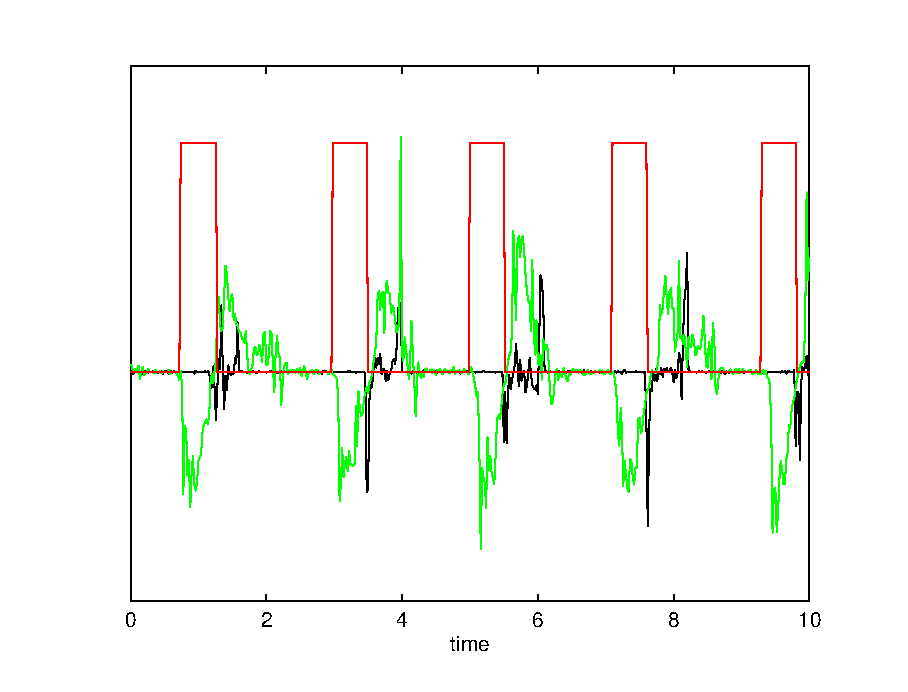
\includegraphics[width=0.48\linewidth]{grasp_seq_scotch.eps} &
      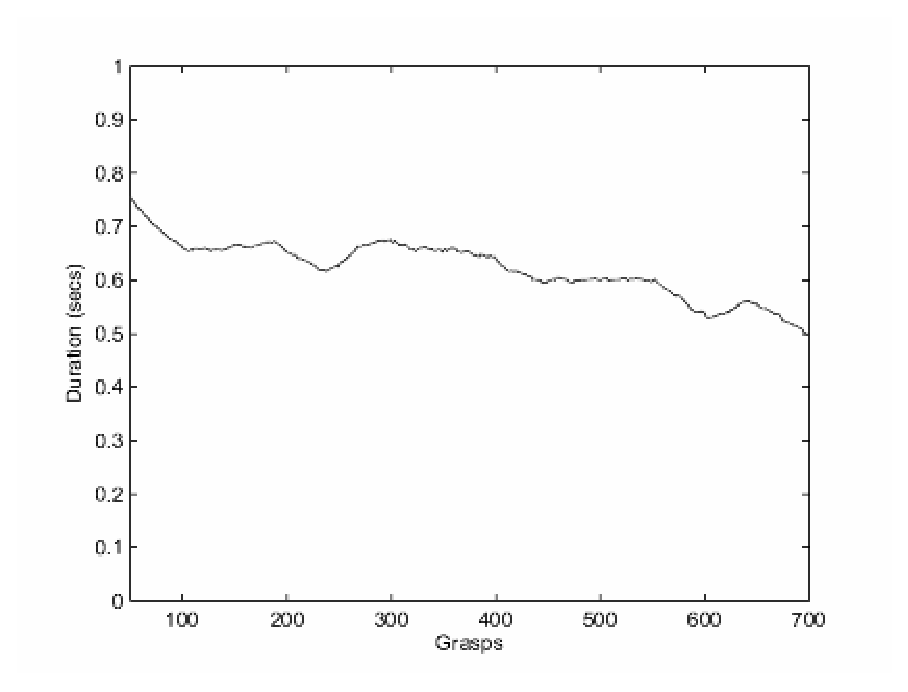
\includegraphics[width=0.48\linewidth]{grasp_trend.eps} \\
      $(a)$ & $(b)$
    \end{tabular}
    \caption{$(a)$ Detecting the grasps. The Figure shows $10$ seconds
    of a subject grasping an object. The red bands indicate the start
    and end of a grasp; the black line is the FSR response; and the
    green line is the hand speed. As one can see, the ending points
    are found near the FSR spike, indicating contact; moreover, the
    hand speed shows the well known bell-shaped curve during a
    grasp. $(b)$ Grasps duration. The Figure shows the duraton of the
    grasps (moving average over 50 grasps) averaged for all
    subjects. As the experiments advance, the duration becomes shorter
    and shorter.}
    \label{fig:grasp_sequence}
  \end{center}
\end{figure}

Overall, the procedure could recognise $716 \pm 12$ grasps for each
subject, which matches the desired result of $720$ ($120$ per session,
each user running six sessions). During two of the experiments, the
FSR sensor broke down, resulting in the procedure recognising $550$
and $649$ grasps in those cases. All data were also manually observed
in order to verify that spurious detected grasps would be an
insignificant fraction of the total grasps.

\subsubsection*{Grasping speed}

In general, in order to make time sequences suitable for a machine
learning system, they all must have the same length;\footnote{An
alternative possibility appears, e.g., in
\cite{shimodaira02dynamic}; this issue is the subject of future
research.} in order to do this, since in general not all grasps have
the same length, we stretched each sequence to a predefined
length. The predefined length was chosen according to the average
speed of the grasps. Figure \ref{fig:grasp_sequence} $(b)$ shows the
average grasp durations for all subjects over each experiment (moving
average over $50$ grasps); as one would expect, in general the
subjects get rapidly used to the grasp/drop/reposition task and the
grasps become faster and faster. It must be remarked, though, that
this is not the case for all subjects considered one by one.

On average, the grasp duration was $0.62 \pm 0.20$ seconds. We decided
then to stretch every grasp to $1$ second by linear interpolation,
obtaining fixed-length time sequences of $50$ samples for each sensor
and grasp.

\subsection{Support Vector Machines}

Our machine learning system is based upon Support Vector Machines
(SVMs). Introduced in the early 90s by Boser, Guyon and Vapnik
\cite{BGV92}, SVMs are a class of kernel-based learning algorithms
deeply rooted in Statistical Learning Theory \cite{v-edbed-82}, now
extensively used in, e.g., speech recognition, object classification
and function approximation with good results \cite{Cristianini00}.

We are interested here in the problem of SVM regression, that is:
given a function whose value is known only for a finite number of
points in its input domain, find its best approximation $f$ drawn from
a suitable functional space $\mathcal{F}$. In practice, let
$S=\{\xx_i,y_i\}_{i=1}^l$, with $\xx_i \in \RR^m$ and $y_i \in \RR$ be
a set of $l$ points and output values of the unknown function
(actually, the training set); then the resulting $f(\xx)$ is a sum of
$l$ elementary functions $K(\xx,\yy)$, each one centered on a point in
$S$, and weighted by real coefficients $\alpha_i$:

\begin{equation} \label{eqn:sol}
  f(\xx) = \sum_{i=1}^l \alpha_i y_i K(\xx,\xx_i) + b
\end{equation}

\noindent where $b \in \RR$. The choice of $K$, the so-called
\emph{kernel}, is done \emph{a priori} and defines $\mathcal{F}$ once and for
all; it is therefore crucial. According to a standard practice (see,
e.g., \cite{Cristianini00}) we have chosen a \emph{Gaussian} kernel,
which has one positive parameter $\gamma \in \RR$ defining the
standard deviation of the Gaussian functions used to build
(\ref{eqn:sol}).

Let $C \in \RR$ be a positive parameter; then the $\alpha_i$s and $b$
are found by solving the following minimisation problem
(\emph{training phase}):

\begin{equation} \label{eqn:svm_primal}
  \min \left( R(S) + C \sum_{i=1}^l L^\epsilon (x_i,y_i,f) \right)
\end{equation}

\noindent where $R(S)$ is a \emph{regularisation term} and
$L^\epsilon (x_i,y_i,f)$ is a \emph{loss functional}. Minimising the
sum of $R$ and $S$ together, rather than just the loss functional,
ensures that the solution will approximate well the values in the
training set, at the same time avoiding overfitting, i.e., exhibiting
poor accuracy on points outside the training set. In SVM regression,
$L^\epsilon (x_i,y_i,f) = \mbox{max}(0,|y_i-f(x_i)|-\epsilon)$,
where $\epsilon > 0$ controls the width of an ``insensitive band'' around
the output values, e.g., errors on the training set within this band
are neglected.

There are therefore three parameters to be tuned in our setting:
$C$, $\gamma$ and $\epsilon$. In all our regression tests, we found
$C$ and $\gamma$ by grid search, whereas $\epsilon$ was chosen
according to the resolution of the sensors being examined (see next
Section for a deeper discussion).

Notice, lastly, that the quantity to be minimised in Equation
(\ref{eqn:svm_primal}) is convex; due to this, as well as to the use
of a kernel, SVMs have the advantages that their training is
guaranteed to end up in a global solution and that they can easily
work in highly dimensional, non-linear feature spaces, as opposed to
analogous algorithms such as, e.g., artificial neural networks. For an
extensive introduction to regression based upon SVMs, see, e.g.,
\cite{SmolaTut2004}. Our system employs LIBSVM v2.82 \cite{ChangL01},
a standard, efficient implementation of SVMs.

According to the procedure described in the previous parts of this
Section, we decided to define $\RR^{50}$ as the input space of our
machines, and to use, for each sensor in the setup, the stretched
grasping sequences as points; the target values would then be the
values of the same sensor at the time of contact with the object. This
way we have obtained $28$ SVMs, each one approximating the value of a
sensor at the time of contact.


\section{RESULTS}
\label{sec:exp_res}
Our machine learning system is based upon Support Vector Machines
(SVMs). Introduced in the early 90s by Boser, Guyon and Vapnik
\cite{BGV92}, SVMs are a class of kernel-based learning algorithms
deeply rooted in Statistical Learning Theory \cite{v-edbed-82}. As
opposed to analogous algorithms such as, e.g., artificial neural
networks, they have the main advantages that their training is
guaranteed to end up in a global solution, that they can easily work
in highly dimensional, non-linear feature spaces, and that the
solution achieved is sparse. Due to these good properties, they have
been now extensively used in, e.g., speech recognition, object
classification and function approximation with good results
\cite{Cristianini00}. For an extensive introduction to regression
based upon SVMs, see, e.g., \cite{SmolaTut2004}. Our system employs
LIBSVM v2.82 \cite{ChangL01}, a standard, efficient implementation of
Support Vector Machines.

We were mainly interested in answering two questions:

\begin{enumerate}

  \item how far in the future can our system predict well?

  \item how does the knowledge of the grasped object affect the error?

\end{enumerate}

In order to answer the first question, we have set up a regression
experiment in which a \emph{blind fraction} $0 \leq B \leq 1$ of the
grasp was taken as main parameter. $B$ indicates what fraction of the
data associated to the grasp, from the contact point backwards, is
hidden to the system. In practice, since the sampling frequency was
$50$Hz and each grasp was stretched to $1$ second, a sequence of
$(1-b)*50$ samples was fed to the SVM, along with the desired value as
target. This procedure was repeated for each single sensor. At the
end, the overall error was obtained by grouping the $28$ sensors this
way: the $3$ numbers representing the position of the hand (coming
from the FoB), the $3$ numbers representing the orientation of the
hand (coming from the FoB too), and the $22$ numbers representing the
posture of the hand (coming from the DataGlove). According to the
device resolutions detailed in the previous Section, we set the
$\epsilon$ value related to the SVM \cite{SmolaTut2004} like this:
$0.1$ inches for each component of the hand position, $0.5$ degrees
for each component of the hand orientation and $1$ degree for each
component of the hand posture. As an ``acceptable'' error, we
considered approximately two or three times this value.

As far as the Support Vector Machines are concerned, a Gaussian kernel
was chosen, and its hyperparameters ($C$ and $\gamma$) were found by
grid search. The error on regression was obtained by $5$-fold
cross-validation. This ensures a good degree of generalisation.

\subsubsection*{Overall accuracy}

\subsubsection*{Accuracy given an object}

\subsubsection*{Discussion}



\section{DISCUSSION}
\label{sec:Conclusions}
With this initial experiment we really pose further questions and
sketch future research rather than draw definite conclusions. The
machine learning questions addressed in this paper do indeed have an
answer, albeit partial; on the other hand, it remains difficult to say
something other than speculations when comparing these results to
neuroscience.

In short, the answer to the two questions posed in Section
\ref{sec:exp_desc} is that we can predict well given that we have
access to motor information at least during learning, and that knowing
the objects to be grasped improves the ability to predict the outcome
of an action. There are many caveats in this experiment, as for
example, the question on whether a pre-processing of the data through
clustering could improve performance further: i.e., given that objects
afford certain grasping postures and they are executed with high
probability. In humans the quality of the prediction of grasping is a
function of the expectancies of the various possible grasp types which
are in turn determined by the past experience of manipulation of the
target object\footnote{personal communication with Luciano Fadiga.}.

The solution found by the SVMs detailed in the previous Section is
optimal, since the dependence from hyperparameters has been optimized
out in our case by grid search and cross-validation that although
expensive is known to provide good results. An analysis of the
solution should thus provide an accurate characterization of the
problem qua the data set that has been collected.

In this sense (and only in this sense) we have shown that by
partitioning the training set per object provides a general
improvement of the quality of the solution and simultaneously of the
training time (worst case $O(l^3)$ versus $O(3 \cdot (l/3)^3)$ in our
case with $3$ objects and $l$ the total number of samples). This can
be an effective strategy when the world affords such an intuitive
partitioning as for objects (seen as discrete entities).

This is also true from what is known about the brain structures that
control grasping where the presence of a target object, its shape and
affordance, and in general any contextual cue, are coded separately by
different populations of neurons and influence simultaneously the
response of the neurons that enact specific motor plans. After motor
prediction is in place, the next step, that of recognizing the action
of another individual is conceptually simple since it amounts to
building a classifier on highly predictable motor trajectories.

Another interesting question that is left to future research is
whether we can investigate the complexity of the controllers of
reaching and grasping (which are known to develop separately in
humans) from the complexity of the learned internal models or as a
consequence of the prediction error.

Clearly, the fact that we can train such internal models is prone to
be applied in various contexts, as we mentioned, ranging from control
of robots through interpretation and prediction of human behavior in
particular for man-machine communication.


{\small
\bibliographystyle{alpha}
\bibliography{paper}
}

\end{document}
